\newpage
\section{Existing solutions}
\label{sec:altsolution}

To get a full impression of what functionality our product should have, the team did some research on similar solutions that already existed on the market. The research was based on the product requirements the team worked out with the customer, resulting in a list of the most relevant solutions.
 
This list contains a brief overview of the functionalities and drawbacks of existing solutions, summarized in table~\ref{tab:existingSolutions}. The team used this study in alternative solutions as an inspiration for functionality and features to implement in the project app.


\begin{table}[H]
\centering
\rowcolors{1}{darkgray}{lightgray}
\begin{tabular}{|l|l|p{2.6cm}|p{2.3cm}|p{2.2cm}|}
\hline
\textbf{Product} & \textbf{Device control} & \textbf{Social media} & \textbf{Measure production} & \textbf{Measure individual devices} \\
Smartly & Limited & No  & No & No\\
OpenEnergyMonitor & Yes & No  & Limited & No \\
Minisolo & Yes & No  & No & Limited\\
TheOwl & Yes & No & No & Yes\\
Efergy & Yes & Yes &  No & Yes\\\hline
\end{tabular}
\caption{Comparison of existing solutions}
\label{tab:existingSolutions}
\end{table}


\subsection{NTE miniSolo energydisplay}

The NTE miniSolo energydisplay~\cite{nte} measures the total power usage real time and allows the user to power off devices to see the effect the device has on the total power consumption. It offers some interesting features like detailed power consumption and an overview of how much money the power usage amounts to. However, the miniSolo energydisplay has some drawbacks: It is linked to a proprietary device, and it has no Android app. These drawbacks made the solution incompatible with the team's project.


\subsection{Theowl}

Theowl~\cite{theowl} mainly focuses on temperature control. This was a drawback because the team would like to focus on other properties, such as controlling individual devices. The product does not have any official support in Norway, and it is not within a reasonable price range. 

However, Theowl has an architecture with remote sensors that sends precise data and allow the user to control certain devices, which the team would like to consider for the project.


\subsection{Smartly}

Smartly~\cite{smartly} allows the user to monitor and control things like temperature and lighting in the house, as shown in figure~\ref{fig:smartlya}. It also has an overview over the total power consumption, as shown in figure~\ref{fig:smartlyb}.

Smartly has several interesting features and concepts, such as being able to turn on and off certain devices, and functionality for displaying money saved. The graphical user interface is also well designed and user friendly. It does however lack the functionality to monitor the power usage of single devices.

\begin{figure}[H]
\addcontentsline{lof}{figure}{2.1\hspace{4mm}Smartly screenshots}
\label{fig:smartly}
  \centering
  \subbottom[\label{fig:smartlya}Screenshot of Smartly's possibility to remotely control devices]{
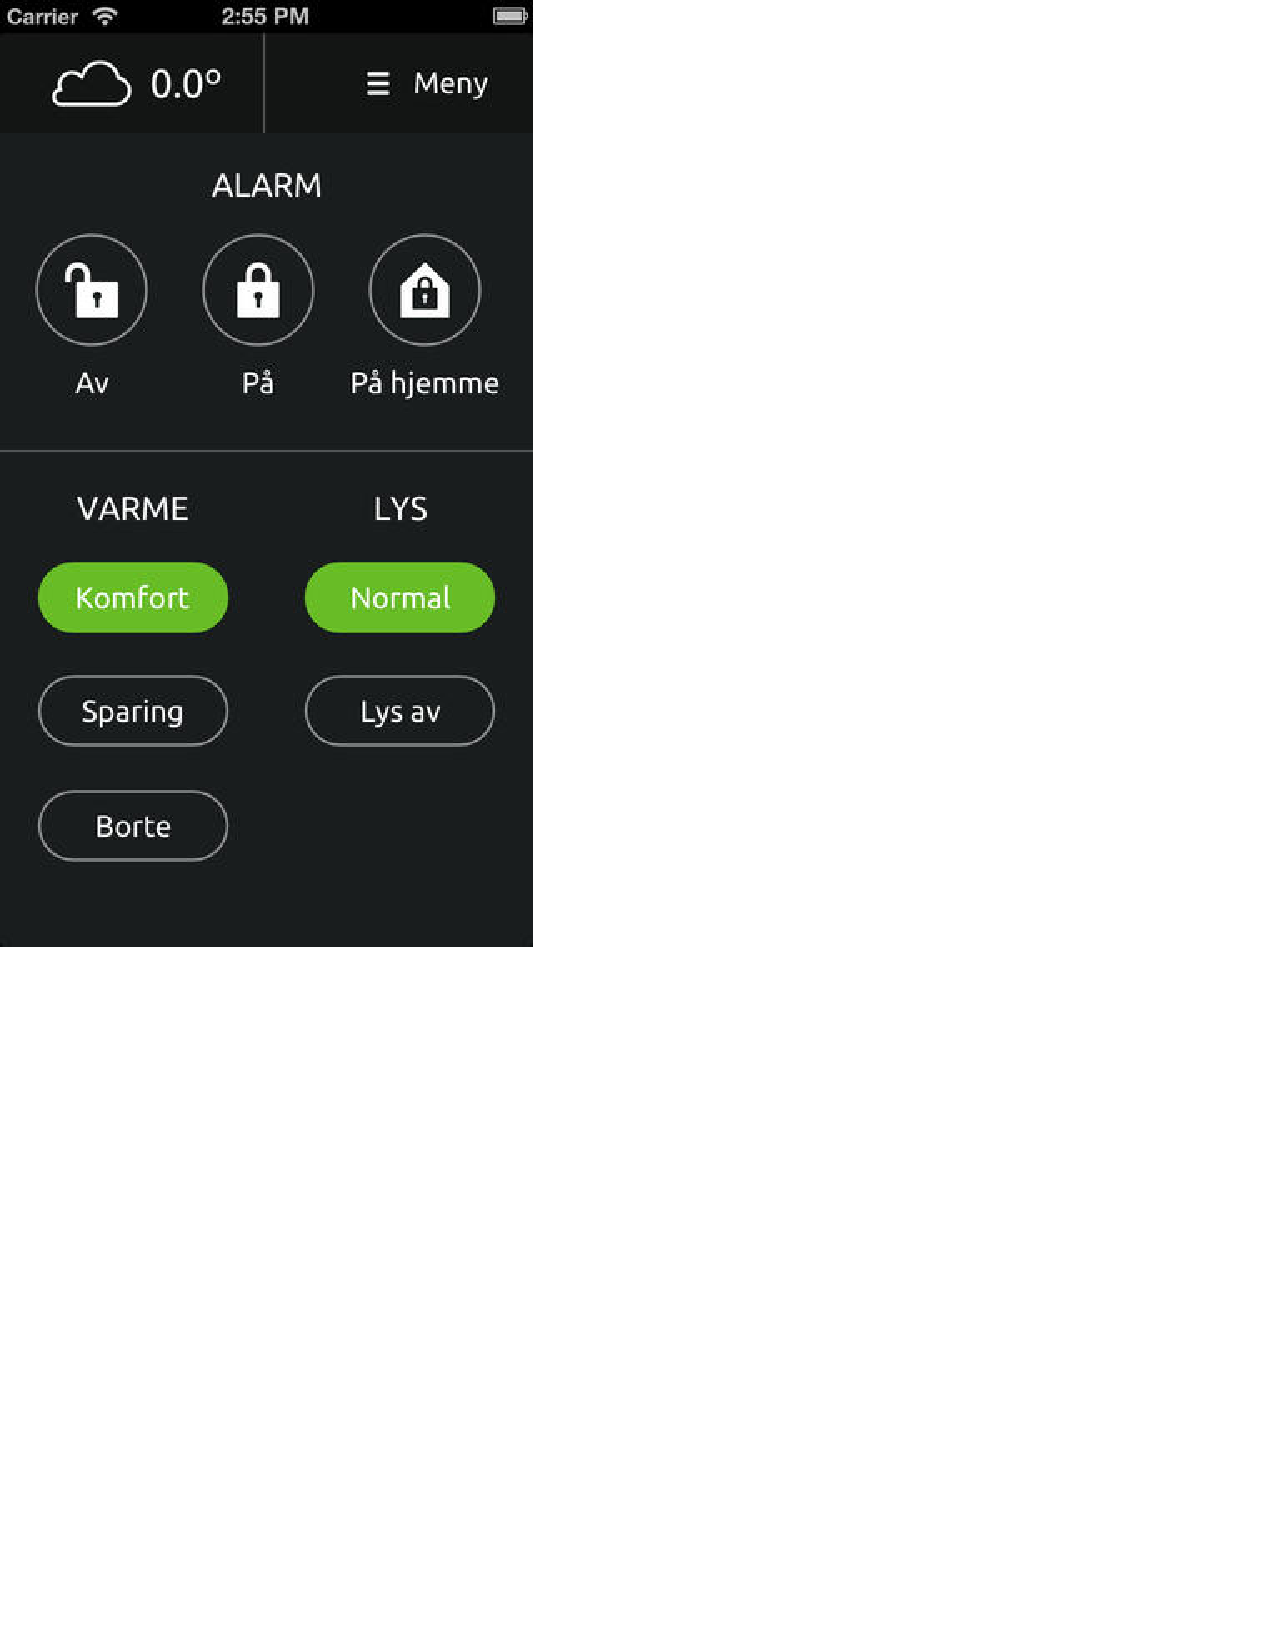
\includegraphics[width=0.35\textwidth, trim=0cm 12cm 13cm 0cm, clip]{ch/prestudy/fig/smartlyLock.pdf}}
\quad
  \subbottom[\label{fig:smartlyb} Screenshot of Smartly's consumption overview]{%
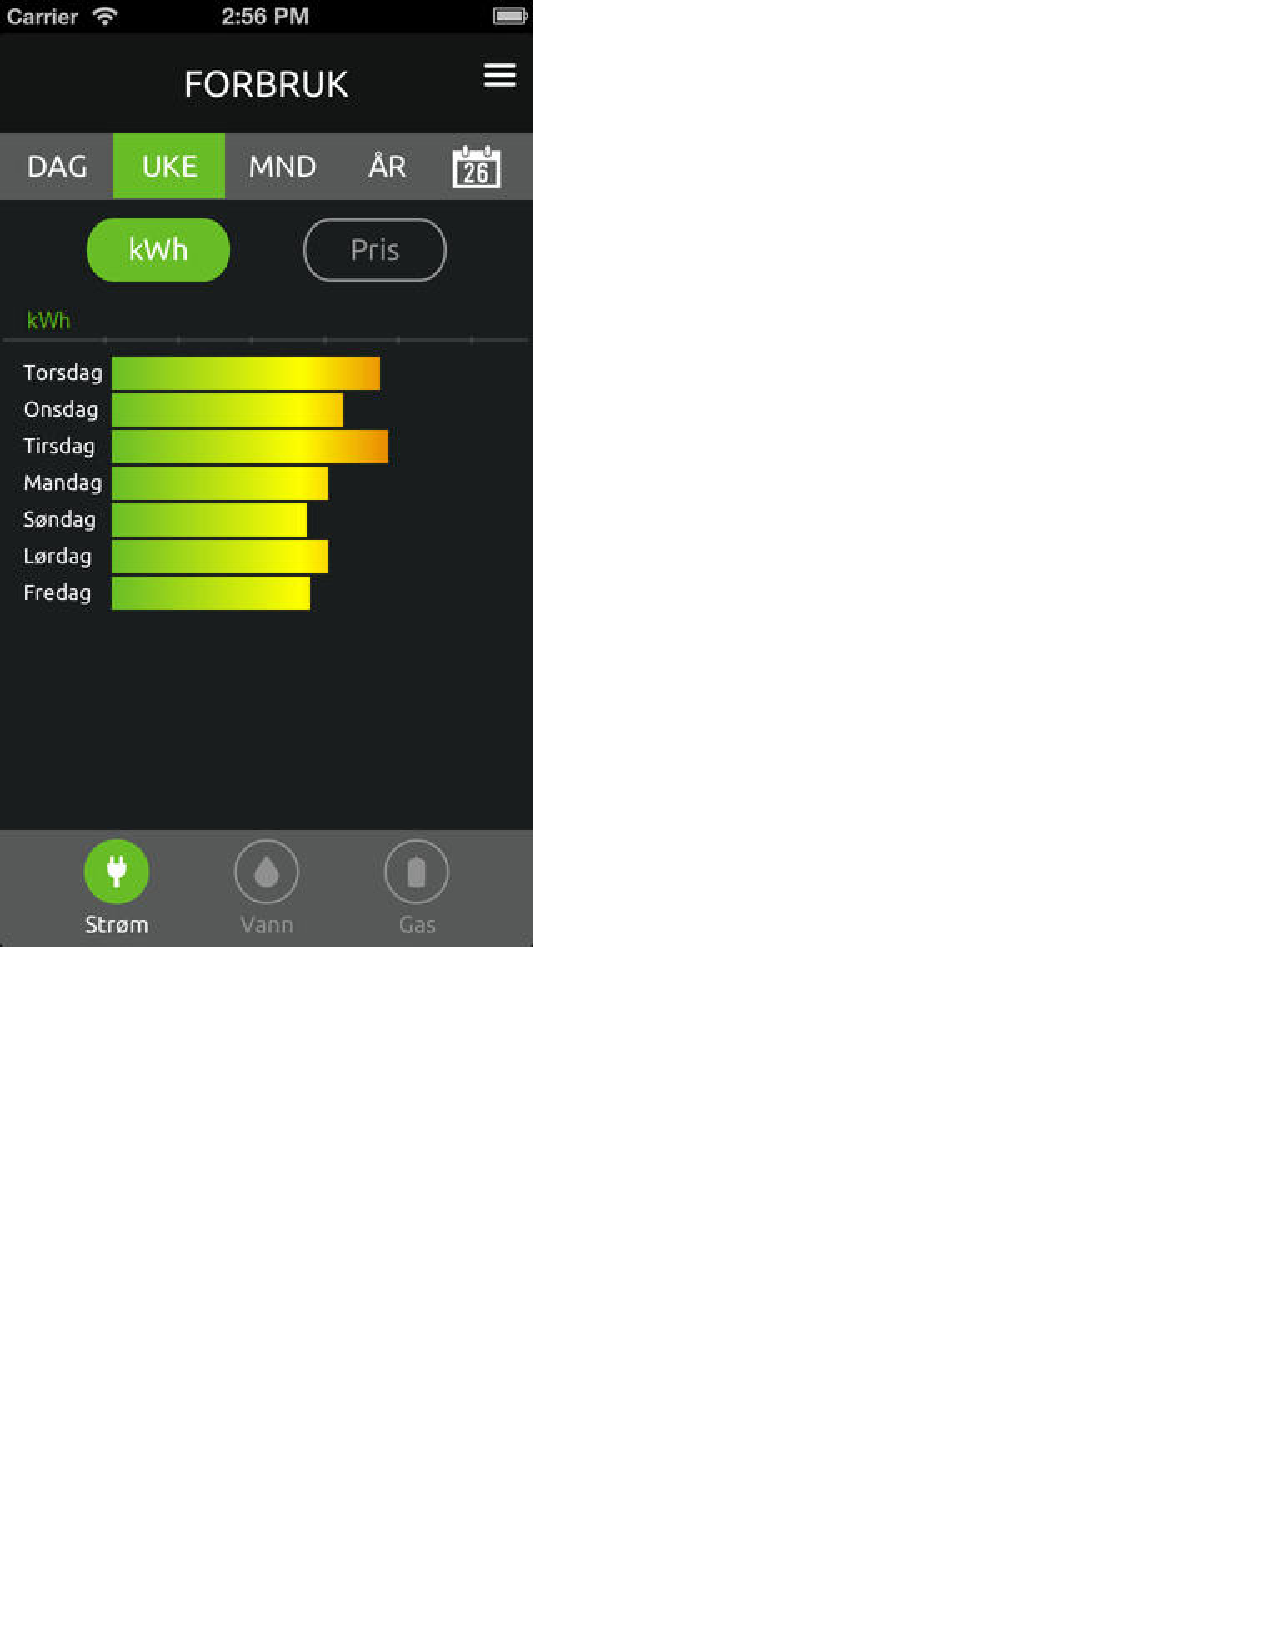
\includegraphics[width=0.35\textwidth, trim=0cm 12cm 13cm 0cm, clip]{ch/prestudy/fig/smartlyConsume.pdf}}
\caption{Screenshots from the Smartly solution}
\end{figure}

\newpage
\subsection{OpenEnergyMonitor}
\label{sec:openenergymonitor}
OpenEnergyMonitor~\cite{openenergymonitor} is an open source project that allows data collection from power outages. Some of the architecture for collecting data can, with some improvements, be an interesting option to consider. The architecture, shown in figure~\ref{fig:oem}, is somewhat similar to what the team imagined using in the project. This solution also has an application for processing, logging and visualizing energy usage.

However, OpenEnergyMonitor offers no automatic collection of data - the user would have to manually collect it. This solution is somewhat hard to set up, and also not very user friendly for the average consumer. 

\setcounter{figure}{1}
\begin{figure}[H]
\centering
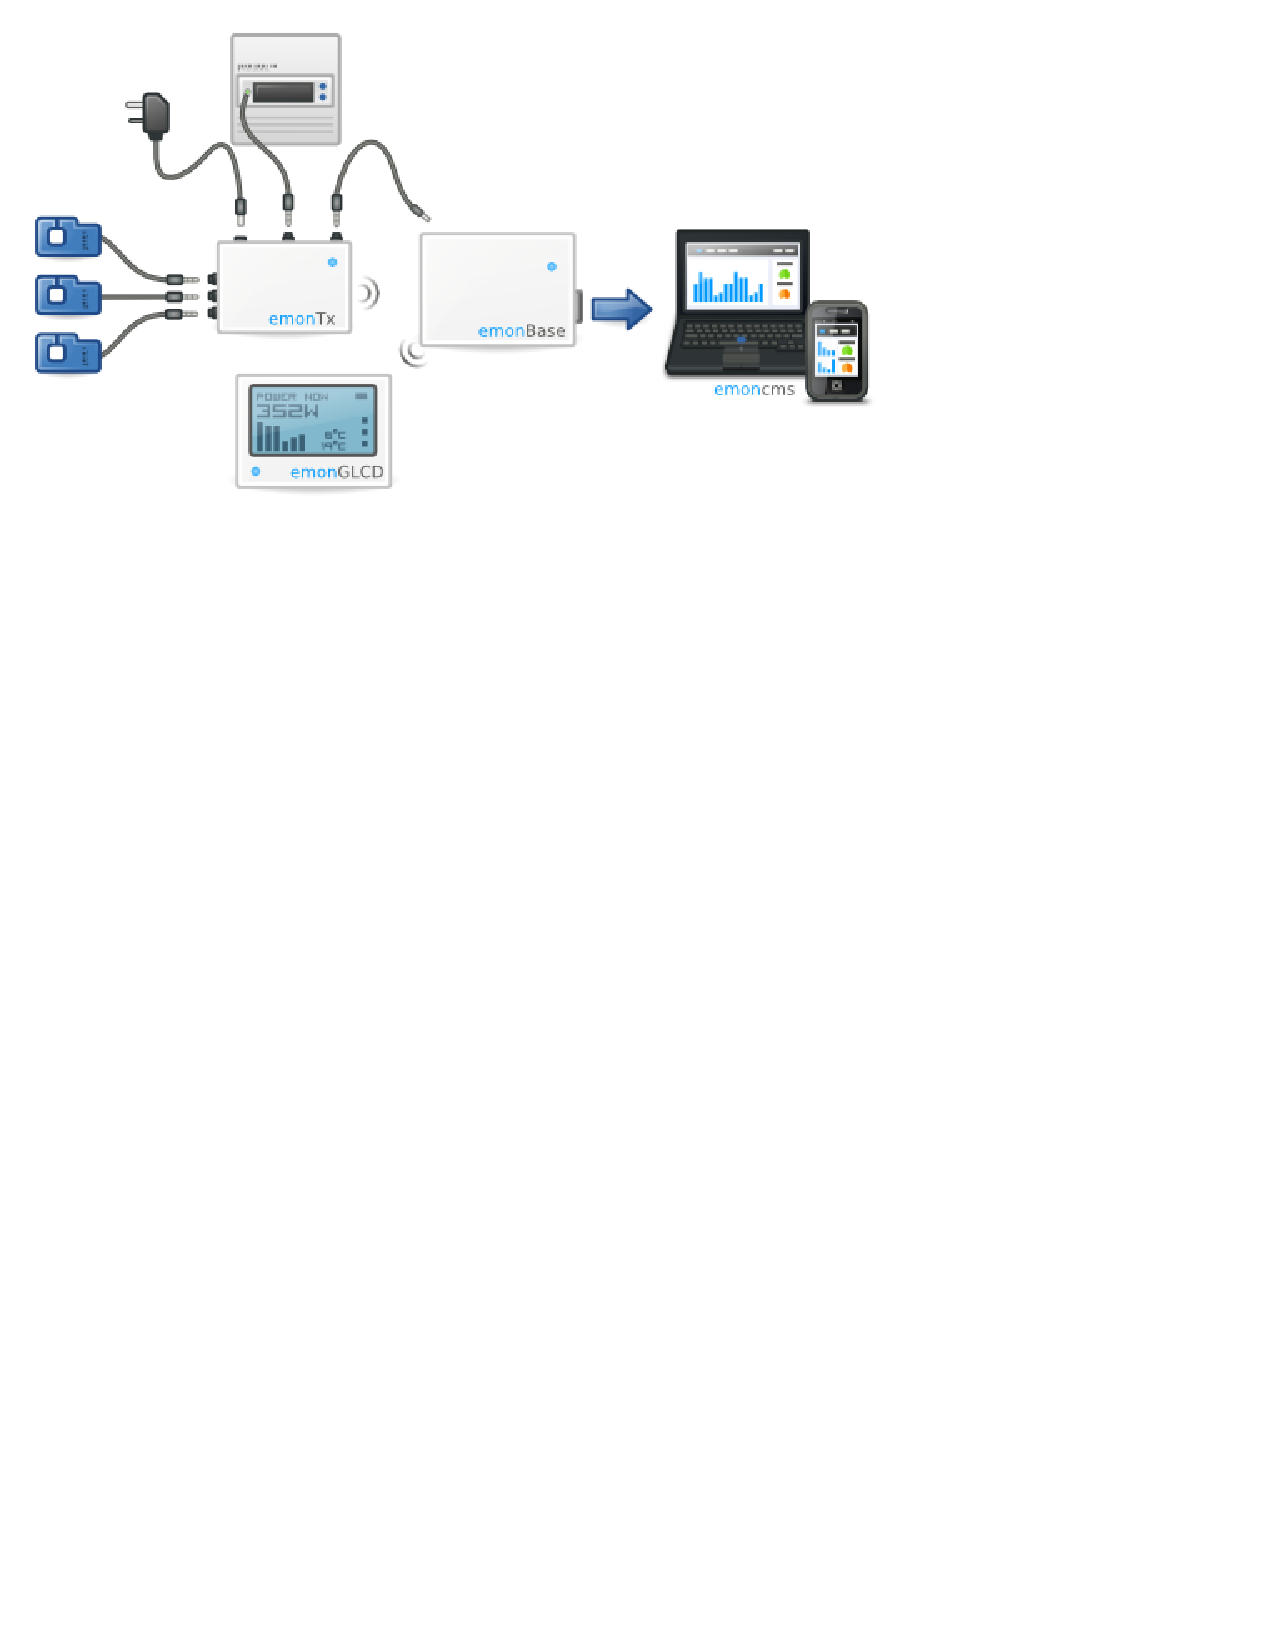
\includegraphics[width=\textwidth, trim=0.5cm 19cm 6.5cm 0cm, clip]{ch/prestudy/fig/OEM_system.pdf}
\caption{OpenEnergyMonitor's system architecture}
\label{fig:oem}
\end{figure}

\newpage
\subsection{Efergy}

Efergy~\cite{efergy} was considered to be the solution that was closest to what the team wanted to develop. As shown in figure~\ref{fig:efergyGUI}, it has a nice visual representation of data, and it offers social integration. The architecture is interesting, as it supports measuring the power usage of single devices. There is a local receiver collecting data from the devices and sending it to a server on the Internet. Unfortunately, this solution lacks the ability to monitor and control private power production. It is also beyond a reasonable price range.

\begin{figure}[H]
\centering
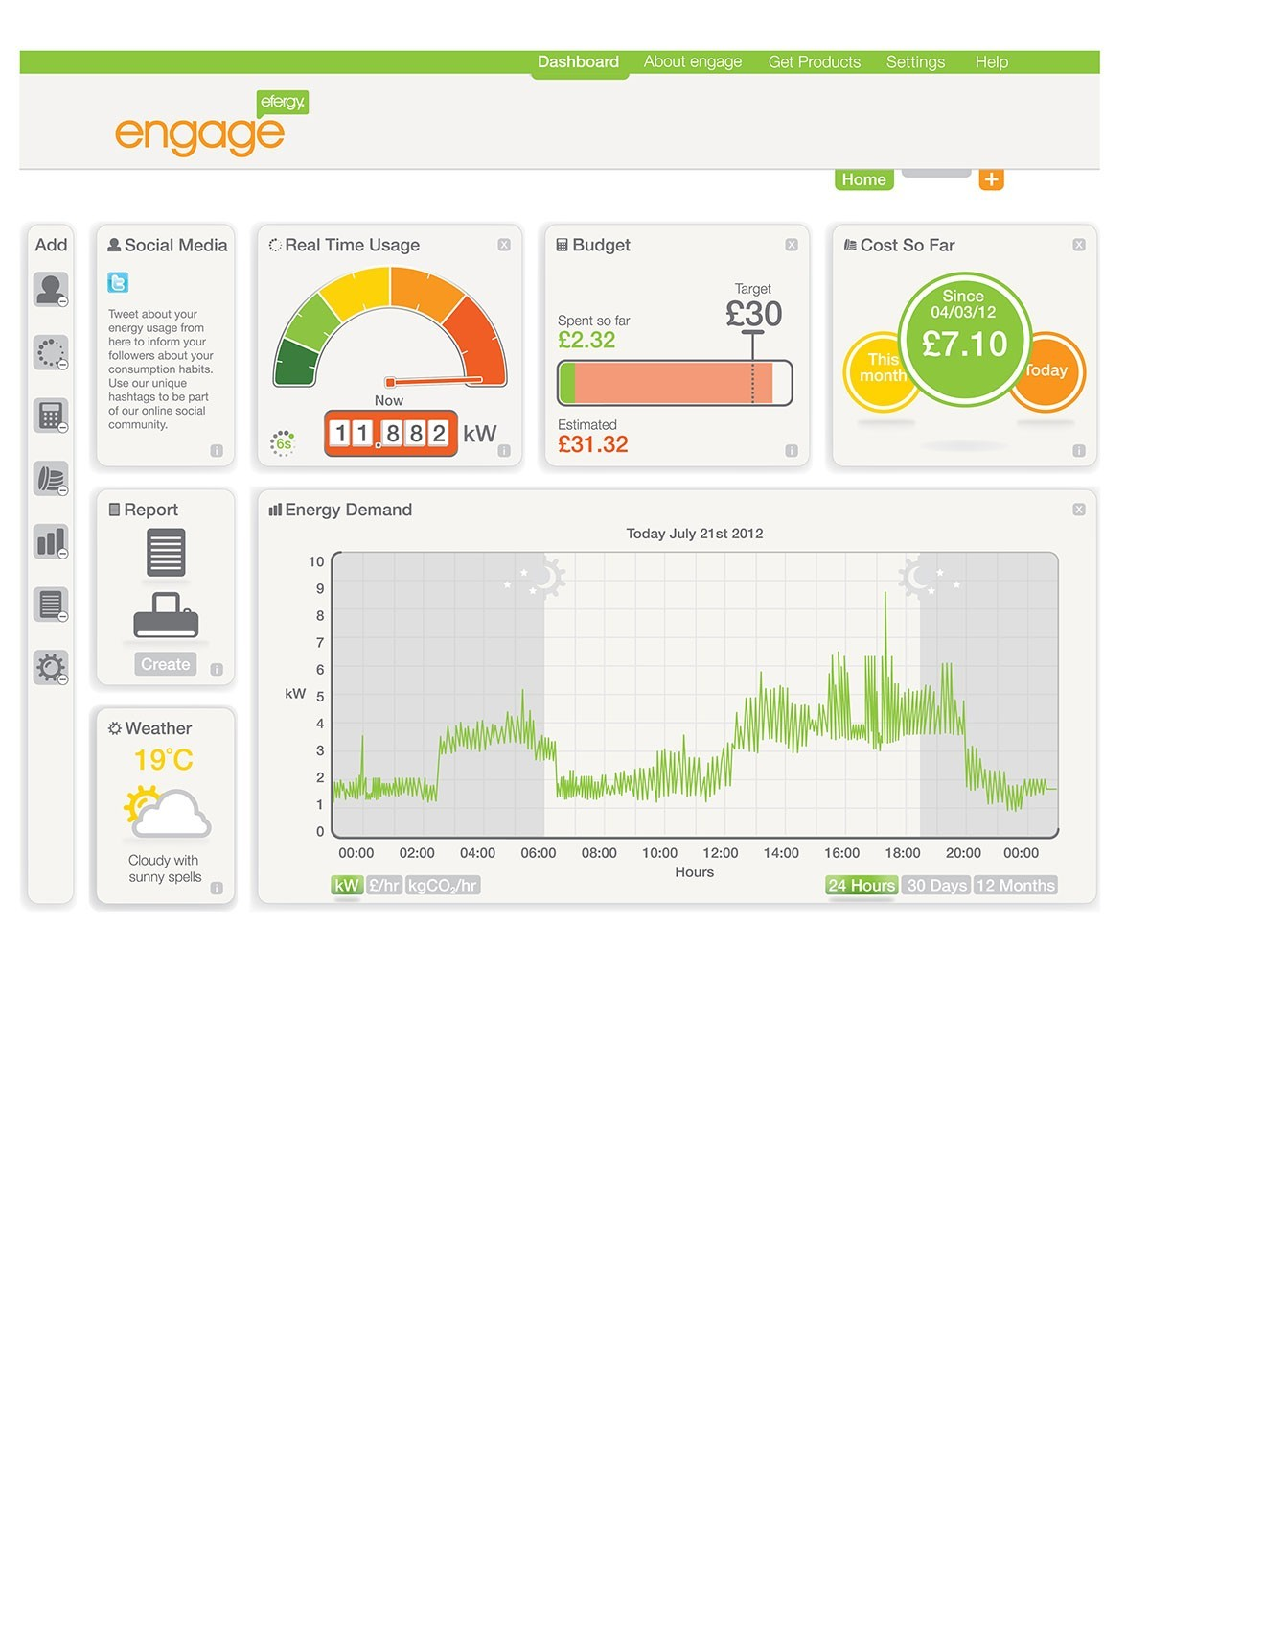
\includegraphics[width=13cm, trim=0.4cm 12cm 3cm 0.7cm, clip]{ch/prestudy/fig/efergy.pdf}
\caption{Screenshot of the Efergy Engage GUI}
\label{fig:efergyGUI}
\end{figure}
